\documentclass[14pt]{extbook}
\usepackage{multicol, enumerate, enumitem, hyperref, color, soul, setspace, parskip, fancyhdr} %General Packages
\usepackage{amssymb, amsthm, amsmath, bbm, latexsym, units, mathtools} %Math Packages
\everymath{\displaystyle} %All math in Display Style
% Packages with additional options
\usepackage[headsep=0.5cm,headheight=12pt, left=1 in,right= 1 in,top= 1 in,bottom= 1 in]{geometry}
\usepackage[usenames,dvipsnames]{xcolor}
\usepackage{dashrule}  % Package to use the command below to create lines between items
\newcommand{\litem}[1]{\item#1\hspace*{-1cm}\rule{\textwidth}{0.4pt}}
\pagestyle{fancy}
\lhead{Progress Quiz 4}
\chead{}
\rhead{Version C}
\lfoot{9187-5854}
\cfoot{}
\rfoot{Spring 2021}
\begin{document}

\begin{enumerate}
\litem{
Which of the following equations \textit{could} be of the graph presented below?
\begin{center}
    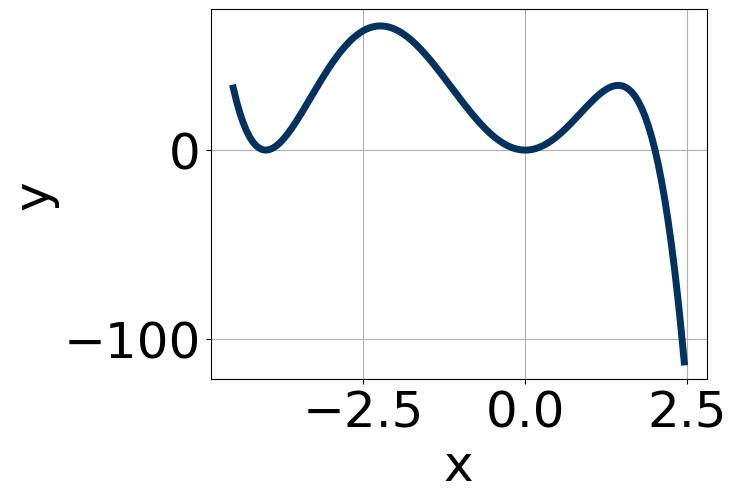
\includegraphics[width=0.5\textwidth]{../Figures/polyGraphToFunctionCopyC.png}
\end{center}
\begin{enumerate}[label=\Alph*.]
\item \( -18(x - 3)^{4} (x - 1)^{6} (x + 3)^{9} \)
\item \( 13(x - 3)^{8} (x - 1)^{9} (x + 3)^{6} \)
\item \( -8(x - 3)^{4} (x - 1)^{5} (x + 3)^{7} \)
\item \( 10(x - 3)^{6} (x - 1)^{9} (x + 3)^{11} \)
\item \( -19(x - 3)^{5} (x - 1)^{10} (x + 3)^{5} \)

\end{enumerate} }
\litem{
Describe the end behavior of the polynomial below.\[ f(x) = -3(x - 3)^{5}(x + 3)^{6}(x - 2)^{3}(x + 2)^{5} \]\begin{enumerate}[label=\Alph*.]
\begin{multicols}{2}\item 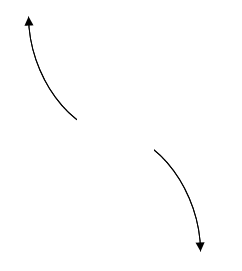
\includegraphics[width = 0.3\textwidth]{../Figures/polyEndBehaviorCopyAC.png}\item 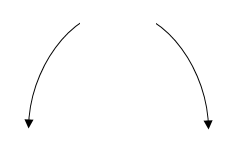
\includegraphics[width = 0.3\textwidth]{../Figures/polyEndBehaviorCopyBC.png}\item 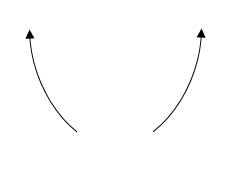
\includegraphics[width = 0.3\textwidth]{../Figures/polyEndBehaviorCopyCC.png}\item 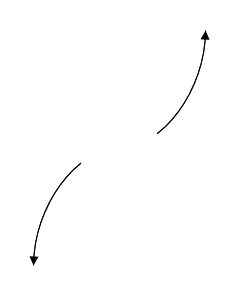
\includegraphics[width = 0.3\textwidth]{../Figures/polyEndBehaviorCopyDC.png}\end{multicols}\item None of the above.
\end{enumerate} }
\litem{
Construct the lowest-degree polynomial given the zeros below. Then, choose the intervals that contain the coefficients of the polynomial in the form $ax^3+bx^2+cx+d$.\[ 4, -7, \text{ and } \frac{-1}{5} \]\begin{enumerate}[label=\Alph*.]
\item \( a \in [4, 10], b \in [53.5, 57.4], c \in [150, 154], \text{ and } d \in [23, 37] \)
\item \( a \in [4, 10], b \in [14.4, 17.4], c \in [-139, -134], \text{ and } d \in [23, 37] \)
\item \( a \in [4, 10], b \in [14.4, 17.4], c \in [-139, -134], \text{ and } d \in [-35, -21] \)
\item \( a \in [4, 10], b \in [-17.7, -14.1], c \in [-139, -134], \text{ and } d \in [23, 37] \)
\item \( a \in [4, 10], b \in [-14.4, -12.2], c \in [-147, -141], \text{ and } d \in [-35, -21] \)

\end{enumerate} }
\litem{
Describe the zero behavior of the zero $x = 9$ of the polynomial below.\[ f(x) = 2(x - 8)^{12}(x + 8)^{8}(x + 9)^{7}(x - 9)^{4} \]\begin{enumerate}[label=\Alph*.]
\begin{multicols}{2}\item 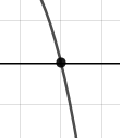
\includegraphics[width = 0.3\textwidth]{../Figures/polyZeroBehaviorAC.png}\item 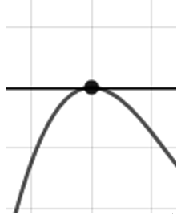
\includegraphics[width = 0.3\textwidth]{../Figures/polyZeroBehaviorBC.png}\item 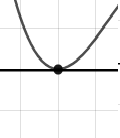
\includegraphics[width = 0.3\textwidth]{../Figures/polyZeroBehaviorCC.png}\item 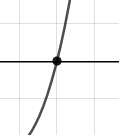
\includegraphics[width = 0.3\textwidth]{../Figures/polyZeroBehaviorDC.png}\end{multicols}\item None of the above.
\end{enumerate} }
\litem{
Describe the end behavior of the polynomial below.\[ f(x) = 8(x + 8)^{2}(x - 8)^{3}(x + 7)^{5}(x - 7)^{7} \]\begin{enumerate}[label=\Alph*.]
\begin{multicols}{2}\item 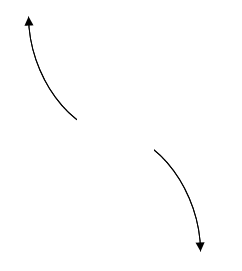
\includegraphics[width = 0.3\textwidth]{../Figures/polyEndBehaviorAC.png}\item 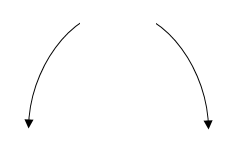
\includegraphics[width = 0.3\textwidth]{../Figures/polyEndBehaviorBC.png}\item 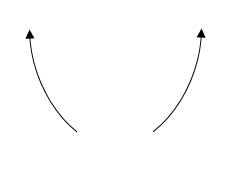
\includegraphics[width = 0.3\textwidth]{../Figures/polyEndBehaviorCC.png}\item 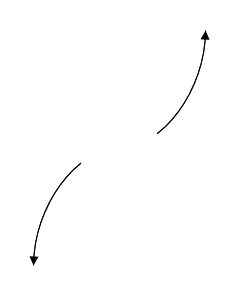
\includegraphics[width = 0.3\textwidth]{../Figures/polyEndBehaviorDC.png}\end{multicols}\item None of the above.
\end{enumerate} }
\litem{
Construct the lowest-degree polynomial given the zeros below. Then, choose the intervals that contain the coefficients of the polynomial in the form $x^3+bx^2+cx+d$.\[ 2 - 5 i \text{ and } -1 \]\begin{enumerate}[label=\Alph*.]
\item \( b \in [-1.3, 1.7], c \in [5, 12], \text{ and } d \in [4, 6] \)
\item \( b \in [-1.3, 1.7], c \in [-5, 2], \text{ and } d \in [-4, 0] \)
\item \( b \in [-5.6, -2.4], c \in [25, 27], \text{ and } d \in [24, 31] \)
\item \( b \in [2.7, 5.9], c \in [25, 27], \text{ and } d \in [-35, -24] \)
\item \( \text{None of the above.} \)

\end{enumerate} }
\litem{
Which of the following equations \textit{could} be of the graph presented below?
\begin{center}
    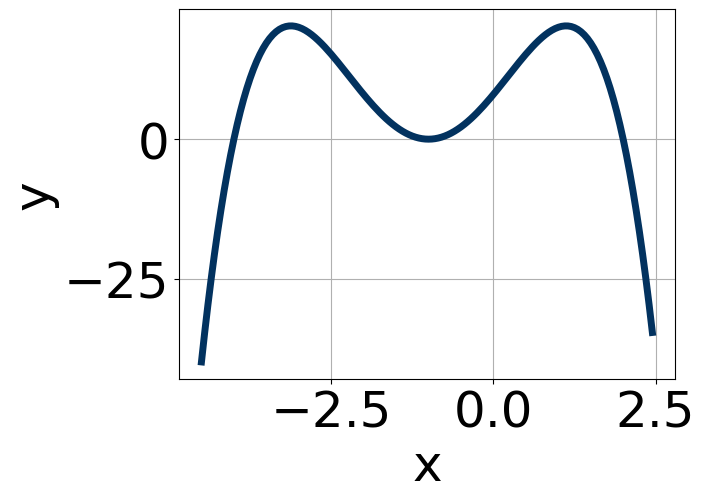
\includegraphics[width=0.5\textwidth]{../Figures/polyGraphToFunctionC.png}
\end{center}
\begin{enumerate}[label=\Alph*.]
\item \( 20x^{8} (x - 3)^{10} (x + 2)^{4} \)
\item \( -11x^{4} (x - 3)^{10} (x + 2)^{6} \)
\item \( -15x^{10} (x - 3)^{6} (x + 2)^{9} \)
\item \( -2x^{6} (x - 3)^{5} (x + 2)^{11} \)
\item \( 17x^{4} (x - 3)^{8} (x + 2)^{7} \)

\end{enumerate} }
\litem{
Construct the lowest-degree polynomial given the zeros below. Then, choose the intervals that contain the coefficients of the polynomial in the form $x^3+bx^2+cx+d$.\[ -4 + 3 i \text{ and } 2 \]\begin{enumerate}[label=\Alph*.]
\item \( b \in [2, 11], c \in [8, 12], \text{ and } d \in [-53, -49] \)
\item \( b \in [-2, 4], c \in [-1, 3], \text{ and } d \in [-10, -6] \)
\item \( b \in [-2, 4], c \in [-5, -3], \text{ and } d \in [6, 8] \)
\item \( b \in [-10, -5], c \in [8, 12], \text{ and } d \in [46, 54] \)
\item \( \text{None of the above.} \)

\end{enumerate} }
\litem{
Describe the zero behavior of the zero $x = 5$ of the polynomial below.\[ f(x) = 5(x + 5)^{7}(x - 5)^{10}(x + 3)^{5}(x - 3)^{6} \]\begin{enumerate}[label=\Alph*.]
\begin{multicols}{2}\item 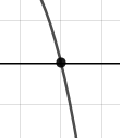
\includegraphics[width = 0.3\textwidth]{../Figures/polyZeroBehaviorCopyAC.png}\item 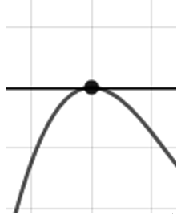
\includegraphics[width = 0.3\textwidth]{../Figures/polyZeroBehaviorCopyBC.png}\item 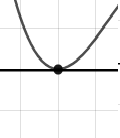
\includegraphics[width = 0.3\textwidth]{../Figures/polyZeroBehaviorCopyCC.png}\item 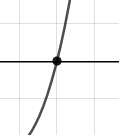
\includegraphics[width = 0.3\textwidth]{../Figures/polyZeroBehaviorCopyDC.png}\end{multicols}\item None of the above.
\end{enumerate} }
\litem{
Construct the lowest-degree polynomial given the zeros below. Then, choose the intervals that contain the coefficients of the polynomial in the form $ax^3+bx^2+cx+d$.\[ 3, 6, \text{ and } \frac{-4}{3} \]\begin{enumerate}[label=\Alph*.]
\item \( a \in [2, 12], b \in [-24, -18], c \in [16, 19], \text{ and } d \in [72, 73] \)
\item \( a \in [2, 12], b \in [-24, -18], c \in [16, 19], \text{ and } d \in [-77, -68] \)
\item \( a \in [2, 12], b \in [20, 24], c \in [16, 19], \text{ and } d \in [-77, -68] \)
\item \( a \in [2, 12], b \in [-12, -2], c \in [-67, -60], \text{ and } d \in [-77, -68] \)
\item \( a \in [2, 12], b \in [27, 34], c \in [90, 95], \text{ and } d \in [72, 73] \)

\end{enumerate} }
\end{enumerate}

\end{document}